\documentclass{report}

%\usepackage{times}
\usepackage[pdftex,
  colorlinks=true,
  pdfstartview=FitV,
  linkcolor=blue,
  citecolor=blue,
  urlcolor=blue]{hyperref}
\usepackage{geometry}
\geometry{a4paper}
\usepackage{amssymb}
%\usepackage{epstopdf}
\usepackage{xspace}
\usepackage{indentfirst}

\usepackage[francais]{babel}
\usepackage[latin1]{inputenc}
\usepackage[dvips]{graphicx}
\usepackage{array}
\usepackage{multirow}
\usepackage{fancyheadings}
\usepackage[Lenny]{fncychap}
\pagestyle{fancy}
\newcommand{\sauteligne}{\vspace{0.5cm}}
\newcommand{\visidia}{ViSiDiA\xspace}
\newcommand{\berlios}{BerliOs.de\xspace}
\author{}
\date{}

\title{
  \begin{flushright}
    \begin{Huge}
      \begin{textbf}
        Projet \visidia\\
      \end{textbf}
    \end{Huge}
    \rule{\textwidth}{2mm}\\
    \large\rm{Cahier des charges}\\
    \vspace{2cm}
    \begin{textbf}\\
      \underline{Auteurs} :\\
      \vspace{0.5cm}
      \sc Nada Ayad\\
      Damien Cassou\\
      Xavier Durand\\
      Jean-Baptiste Gautron\\
      Hicham Ghriss\\
      Mathieu Hopmann\\
      Julie Quagliozzi\\
      \vspace{5mm}
    \end{textbf}
    \rm \today
  \end{flushright}
}

\begin{document}
\maketitle
\tableofcontents

\chapter{R�sum�}

\paragraph{Pr�sentation g�n�rale}

La g�n�ralisation  des r�seaux h�t�rog�nes et de  grandes tailles dans
de   multiples   domaines  implique   des   �tudes  cons�quentes   sur
l'algorithmique    distribu�e.    Le    d�veloppement   d'applications
distribu�es est rendu difficile d�  � des probl�mes de concurrence aux
ressources et � la communication inter processus. C'est la raison pour
laquelle  les chercheurs ont  commenc� �  d�velopper des  logiciels de
simulation.    Ces   logiciels   permettent  de   suivre   l'�volution
d'algorithmes distribu�s graphiquement et en temps r�el dans le but de
comprendre leur fonctionnement, d'en  concevoir de nouveaux mais aussi
dans le but de trouver des propri�t�s et des invariants n�cessaire aux
preuves formelles.


\paragraph{\visidia}

Les chercheurs  du \labri\footnote{Laboratoire Bordelais  de Recherche
  en Informatique}, sous la  direction des professeurs Mohamed Mosbah,
coordinateur  du projet,  et  Yves M�tivier,  responsable de  l'�quipe
algorithmique  distribu�e, ont  mit au  point un  tel  simulateur.  Le
projet \visidia \footnote{Visualization  and Simulation of Distributed
  Algorithms} a pour but de faciliter la visualisation et
la simulation d'algorithmes distribu�s.


\paragraph{Utilisation}

Pour  pouvoir  se  servir  de  \visidia  dans le  but  de  simuler  un
algorithme  distribu�, l'utilisateur  devra commencer  par  �crire son
algorithme    en   utilisant    le   langage    Java   et    une   API
\footnote{Application Programming Interface} de haut niveau fournie et
document�e par  \visidia. Cela fait,  il devra charger ou  dessiner un
graphe   dans  \visidia   puis  pourra   lancer  l'ex�cution   de  son
algorithme. A partir de l�, l'utilisateur visionnera en temps r�el les
diff�rentes actions effectu�es par son algorithme.


\paragraph{Succ�s}

De part son  unique interface � la fois  simple d'utilisation et riche
en  fonctionnalit�s, de  part la  possibilit� de  visualiser  en temps
r�els l'ex�cution  des algorithmes distribu�s  et de part  la pr�sence
d'une  API  puissante  et  simple,   \visidia  est  de  plus  en  plus
utilis�. D'autres  �quipes de chercheurs  l'utilisent et une  �quipe �
Marseille  d�veloppe m�me  le  logiciel.  Les  responsables du  projet
\visidia sont en phase d'installation d'un serveur de gestion de code
source qui  va permettre � plusieurs �quipes  de travailler s�par�ment
sur \visidia tout en permettant l'�volution g�n�rale du logiciel.


\paragraph{Limites}

Il  existe  plusieurs  mod�les  permettant de  g�rer  les  algorithmes
distribu�s.   Le  plus  commun  est  le mod�le  de  communication  par
message.   Chaque  sommet  ex�cute  un algorithme  ind�pendamment  des
autres et  peut aussi communiquer  avec ses voisins.  C'est  le mod�le
implant� actuellement  dans \visidia.  Cependant, ce  mod�le am�ne une
surconsommation des ressources machines  ; en effet, pour chaque noeud
du graphe,  un processus est  cr��.  Si cela  ne pose pas  de probl�me
pour  les petites exp�rimentations,  il est  par contre  impossible de
simuler des algorithmes sur de tr�s gros graphes. C'est en partie pour
cette raison que l'implantation d'un  autre mod�le a �t� envisag�e par
le coordinateur.


\paragraph{Les agents}

Le  mod�le  envisag� par  l'�quipe  du  \labri  est celui  des  agents
mobiles.   Dans  ce mod�le,  les  noeuds  du  graphe n'ex�cutent  plus
d'algorithme, ils  deviennent compl�tement  passifs et ne  peuvent que
stocker des  informations.  Les agents  sont des entit�s  autonomes de
calcul qui se d�placent dans le graphe. Sur chaque sommet, ils peuvent
effectuer  les  actions  qu'ils  d�sirent  comme lire  ou  �crire  des
informations  sur  le sommet,  attendre,  se  dupliquer  etc. puis  se
d�placer  vers  un autre  sommet  et  y  effectuer un  autre  ensemble
d'actions. Il a �t� d�montr� que les deux mod�les sont �quivalents.


\paragraph{Le projet}

Dans le cadre de la formation d'ing�nieurs de l'ENSEIRB\footnote{�cole
Nationale      Sup�rieure     d'�lectronique,      Informatique     et
Radiocommunication  de  Bordeaux},  il  a  �t�  demand�  �  un  groupe
d'�tudiants  d'implanter  le  mod�le  �  base  d'agents  mobiles  dans
\visidia.  Ce projet,  d'une dur�e de quatre mois,  devait se faire en
respectant le  plus possible les proc�dures  habituellement suivie par
l'industrie :  r�daction et validation  par le client d'un  cahier des
charges,  pr�sentation  r�guli�re  de  livrables en  accord  avec  les
attentes du client,  respect de d�lais stricts et  remise d'un rapport
et d'un manuel d'utilisation et d'�volution.


%%% Local Variables: 
%%% mode: latex
%%% TeX-master: "rapport"
%%% TeX-PDF-mode: t
%%% coding: latin-1
%%% End: 

%damien
%pr�sentation du projet et but
\chapter{Domaine d'application}
%%Introduction
%Bases & principes
%
Dans  cette  partie,  On  s'int�resse  aux  bases  de  l'algorithmique
distribu�e. Le contenu de cette  partie ne sera qu'un minimum � savoir
pour aborder  le reste de ce  rapport. Bien qu'on peut  trouver dans ce
qui suit des notions sur  la th�orie des graphes, cette partie suppose
une connaissance consid�rable de certain �l�ments de cette th�orie.
\section{Introduction � l'algorithmique distribu�e}
\subsection{D�finitions}
\subsubsection{R�seau}
On mod�lise un r�seau par  un graphe de mani�re intuitive. Les sommets
repr�sentent les  processeurs, dont l'�tat nous  int�resse par rapport
au r�seau.   Dans un r�seau  synchrone, un top horloge  cadence toutes
les op�rations.  Dans un  r�seau asynchrone, les op�rations peuvent se
produire n'importe o� et quand.
%%%
\begin{figure}[ht]
  \centering
  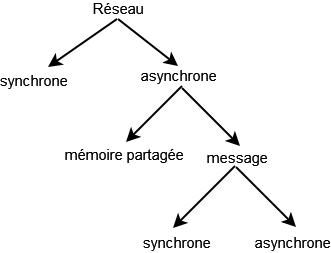
\includegraphics[width=8cm]{figures/algodist.png}
  \caption{Les types des r�seaux en terme de synchronisation, un sch�ma
  pareil peut  �tre �labor� en  s'appuyant sur la connaissance  ou pas
  des noeuds du r�seau}
  \label{fig:algodist}
\end{figure}
\subsubsection{Algorithmique distribu�e}
 La difficult� de  l'algorithmique distribu�e vient essentiellement du
fait  que  chaque  processeur  doit communiquer  uniquement  avec  ses
voisins, � l'aide de registres partag�s, ou par �change de message. De
mani�re g�n�rale,  on d�finit un algorithme distribu�  par un ensemble
de  r�gles  de  transformations  d'�tat  (avec  un  ordre  partiel  de
priorit�).  Si les  transformations induites  par cet  algorithme sont
ind�pendantes, elles sont susceptibles avoir lieu en m�me temps, sinon
on choisit une fa�on non d�terministe la transformation � effectuer.

\subsubsection{Preuve en algorithmique distribu�e}
La preuve d'un tel algorithme se fait en deux temps.  Tout d'abord, on
prouve  la   terminaison  de  l'algorithme,   par  des  consid�rations
combinatoires sur le nombre maximum d'�tapes, qui doit �tre fini. Puis
on   prouve   la  validit�,   le   plus   souvent   en  exhibant   des
invariants... sur lesquels on s'appuie pour r�diger la preuve.
\subsubsection{messages synchrones}
On parle de messages synchrones lorsque l'envoyeur et le receveur sont
synchronis�s, c'est-�-dire  qu'un rendez-vous est mis en  place par un
protocole  (exemple,  le  t�l�phone).  Par  opposition,  on  parle  de
messages  asynchrones  lorsqu'il   y  a  une  d�synchronisation  entre
l'envoyeur et le receveur (exemple, le courrier �lectronique).
%\section{Des principes de base}

\section{Quelques algorithmes simples}
%%%
\subsection{Algorithme de reconnaissance d'un graphe connexe}
On part  d'un sommet que  l'on marque, on  empile ses voisins.  On les
visite,  on les marque  et on  empile les  voisins des  voisins..., Le
graphe est connexe\footnote{Un graphe  (orient� ou non) est connexe si
et  seulement si, pour  tout couple  de sommets,  il existe  une suite
d'ar�tes reliant ces sommets.
\label{grapheConnexe}}  si  tous les  sommets  sont  marqu�s. Pour  la
reconnaissance d'un  graphe fortement connexe,  il convient d'utiliser
deux marques.

\subsection{Algorithme n�1 pour le calcul d'un arbre recouvrant}
Cet  algorithme   permet  le   calcul  d'un  arbre   recouvrant  (sans
reconnaissance locale de la  terminaison globale, cf.  algorithme n�2)
. Consid�rons la r�gle de transformation suivante:

\begin{figure}[ht]
  \centering
  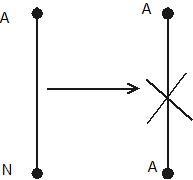
\includegraphics[width=5cm]{figures/algodist1.png}
  \caption{Algorithme n�1: Exemple d'une transformation A-N}
  \label{fig:algodist1}
\end{figure}

On  se donne  un graphe  G. Initialement  tous les  sommets  sont dans
l'�tat Neutre.  On choisit  un premier sommet,  dans l'�tat  Actif. On
applique  les transformations  � partir  de ce  point.  Le sous-graphe
d�fini  par les  ar�tes marqu�es  est  un arbre  recouvrant du  graphe
initial.
\subsection{Algorithme n�2 pour le calcul d'un arbre recouvrant}
Cet algorithme  permet le calcul d'un arbre  recouvrant avec d�tection
locale de la terminaison globale  (�tat F).  Consid�rons les r�gles de
transformation suivantes. R1 a une plus grande priorit� que R2.

\begin{figure}[ht]
  \centering
  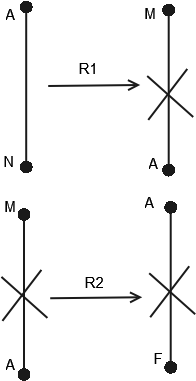
\includegraphics[width=4cm]{figures/algodist2.png}
  \caption{Algorithme n�2  : Exemple d'algorithme � base  de r�gles de
  r��critures}
  \label{fig:algodist2}
\end{figure}

\section{Exemples de probl�mes de l'algorithmique distribu�e}
Dans  le domaine  de l'algorithmique  distribu�es on  trouve  plein de
probl�me qui sont  connus, dans cette partie il  s'agit pas de traiter
ces probl�mes mais juste de donner une id�e sur eux.
\subsection{Le probl�me de l'�lection}
On consid�re  un r�seau ; on  souhaite positionner un  unique noeud du
r�seau dans un �tat �lu et tous les autres dans un �tat non �lu.
\subsubsection{Algorithme dans le cas d'un anneau} 
Soit G un anneau, asynchrone avec �change de messages asynchrones, � 3
�tats :  non �lu,  �lu, ind�fini. Les  sommets sont  initialement dans
l'�tat   ind�finis.  Chaque   processeur  i   du  r�seau   poss�de  un
identificateur   $id_{i}$  unique  (un   entier).  L'anneau   est  orient�,
c'est-�-dire  que  les processeurs  ont  la  notion  de gauche  et  de
droite.   Le  processeur   �lu  est   celui  qui   a  le   plus  grand
identificateur.  Chaque processeur transmet � son voisin de droite son
identificateur. Lorsqu'un processeur re�oit  un identificateur, il y a
trois possibilit�s :
\begin{itemize}
\item Si l'identificateur re�u est plus grand que le sien, il le passe
au suivant (voisin de droite) et passe dans l'�tat non �lu.
\item Si l'identificateur re�u est plus petit que le sien, il jette le
message.
\item Si l'identificateur re�u est le m�me que le sien, alors il prend
l'�tat �lu.
\end{itemize}

\subsection{Probl�mes de reconnaissance}
Peut-on savoir si le r�seau  est un graphe complet, planaire, si c'est
un arbre,  un anneau  ?  Peut-on  savoir encore si  un sommet  est une
articulation, si  une ar�te est un  isthme ?  Dans le  premier cas, il
existe un syst�me de r��criture (ou calcul local) tel que, quand il se
termine, la collecte des  �tiquettes sert de crit�re de reconnaissance
; dans le second cas, ce n'est pas possible !
\subsection{D�tection de la terminaison}
Savoir qu'un protocole distribu� est termin� est souvent difficile. On
peut chercher �  avoir un d�tection locale de  la terminaison globale,
c'est-�-dire qu'un processeur  peut savoir en fonction de  son �tat et
de celui de ces voisins si l'algorithme est termin�.


\section{Quelques applications}
L'algorithmique distribu�e est appliqu� dans plusieurs domaines, Comme
par exemple :
\subsection{Construction d'objets parall�les}
Un exemple des applications dans ce domaine est men� par le PRISM
\footnote{le laboratoire  de recherche en informatique  sur les th�mes
du Parall�lisme, des R�seaux, des Syst�mes et de la Mod�lisation.(voir
http://www.prism.uvsq.fr/)}, il consiste dans la construction d'objets
pour  l'�laboration d'algorithmes  d'alg�bre lin�aire  utilisables par
des architectures � m�moire distribu�e.
\subsection{Le domaine de l'�nergie}
Un  exemple  d'application  dans  ce  domaine  on  le  trouve  au  LAG
\footnote{le Laboratoire    d'Automatique    de   Grenoble    (voir
http://www.lag.ensieg.inpg.fr/)}  ,  et  qui  vise  contrairement  aux
approches  traditionnelles  qui  consistent  � ajuster  la  production
d'�nergie pour  satisfaire �  la demande, �  proposer un  m�canisme de
coop�ration entre sources et charges  de fa�on � satisfaire au mieux �
des crit�res de satisfaction d�finis par un usager. 

\subsection{Autres applications}
L'algorithmique  distribu�e  est pr�sente  partout  o�  on trouve  des
syst�mes   distribu�s,   ces  derniers   sont   devenu  une   solution
incontournable  dans  plusieurs domaines.  Par  exemple  la plupart  des
syst�mes de s�curit�  et de gestion des pannes  utilisent les th�ories
de ce domaine,  ce qui engendre autant de probl�mes  � r�soudre que de
solutions � proposer.


%algorithmique distribu�e
%hicham
\chapter{Analyse de l'existant}
%\input{analyse}
%ViSiDiA + autres simulateurs AD�gents
%damien
\chapter{Introduction au projet}
%\input{intro}
%ViSiDiA/agents
%julie
\chapter{Besions non fonctionnels}
%\input{besoinsNF}
%jb
\chapter{Besions fonctionnels}
%API
%jb
\chapter{Impl�mentation}
%Structures
%nada
\chapter{Limites de l'impl�mentation}
%mathieu
\chapter{Extensibilit�}
%agents sur architecture distribu�e
%gros graphes
%r�gles de r�ecritures
%hicham
\chapter{Exemples de fonctionnement}
%screenshot
%comment on �crit un algo
%xavier
\chapter{Bilan}
%nada

\end{document}

%% Local Variables: 
%% mode: latex
%% TeX-master: t
%% TeX-PDF-mode: t
%% coding: latin-1
%% End:
